O Transmissor/Receptor Assíncrono Universal (\emph{Universal Asynchronous Receiver/Transmitter}, UART), é um periférico de transmissão e recepção de dados usado na comunicação entre dispositivos, sendo esta comunicação realizada de forma serial e assíncrona, ou seja sem a necessidade de transmissão do sinal de clock de referência. Este modo de transmissão faz necessário o uso de apenas duas vias de comunicação uma para a transmissão e outra para a recepção de dados.

\subsection{Padrão da Comunicação}

\begin{figure}[H]
\centering
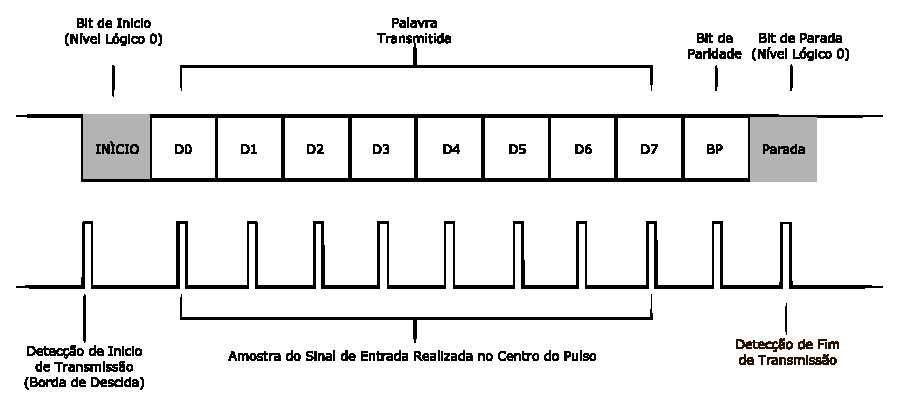
\includegraphics[width=1\textwidth] {figuras/uart.eps}
    \caption{Protocolo de envio na comunicação UART}
    \label{fig:uart}
\end{figure}

Para que a comunicação UART seja realizada é necessário que o sinal de transmissão obedeça a um protocolo. Quando uma palavra é transmitida, primeiro é enviado um bit de início de transmissão para o receptor. Este bit deve ser de nível logico 0 para que a ocorrência da borda de descida sinalize ao receptor que sincronize a amostragem do sinal a ser lido de modo que ela ocorra no meio de cada período de transmissão.  Após transmitir os dados é necessário enviar um bit informando a existência de paridade ou não, e por último é enviado um bit de nível lógico alto para informar o fim da transmissão. Esta sintaxe pode ser observada na figura \ref{fig:uart}.

\subsection{UART do TM4C1294NCPDT}


O Tiva TM4C1294NCPDT possui 4 módulos de comunicação UART. Cada um destes  possuem um gerador de \emph{baud-rate}, ou taxa de transmissão, que possibilitam  transmissões de até 7,5 Mbps em modo de normal transmissão e  15 Mbps em modo \emph{High Speed}. 

Para que seja possível regular o \emph{baud-rate} de forma mais precisa os módulos UART possuem um divisor de 22 bits, sendo 16 bits inteiros e 6 bits fracionários, pelo qual o módulo determina o período de transmissão de bit.

Já o buffer de leitura e transmissão do UART no Tiva tem um tamanho de 8 bits, porém para cada módulo existe uma FIFO de 16x8 bits tanto para transmissão quanto para recepção, sendo que o \emph{trigger} de interrupção de estouro da FIFO é selecionável entre 1/8, 1/4, 1/2, 3/4, 7/8 ou 8/8. 

O sinal de transmissão criado pelo UART do tiva pode transmitir dados seriais de 5,6,7 ou 8 bits de dados precedidos do bit de \emph{Start} e acompanhados de um bit de paridade, se estiver habilitado, e 1 ou 2 bits de parada. A figura \ref{fig:uartTiva} apresenta o sinal característico da transmissão UART do Tiva. 

\begin{figure}[H]
	\centering
	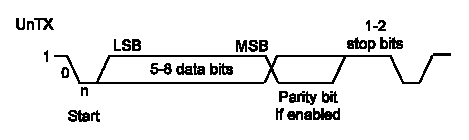
\includegraphics[width=0.5\textwidth] {figuras/uartTiva.eps}
	\caption{Sinal de Transmissão UART no Tiva TM4C1294NCPDT}
	\label{fig:uartTiva}
\end{figure}


\subsection{Na TivaWare}

